\documentclass{article}\usepackage[]{graphicx}\usepackage[]{color}
%% maxwidth is the original width if it is less than linewidth
%% otherwise use linewidth (to make sure the graphics do not exceed the margin)
\makeatletter
\def\maxwidth{ %
  \ifdim\Gin@nat@width>\linewidth
    \linewidth
  \else
    \Gin@nat@width
  \fi
}
\makeatother

\definecolor{fgcolor}{rgb}{0.345, 0.345, 0.345}
\newcommand{\hlnum}[1]{\textcolor[rgb]{0.686,0.059,0.569}{#1}}%
\newcommand{\hlstr}[1]{\textcolor[rgb]{0.192,0.494,0.8}{#1}}%
\newcommand{\hlcom}[1]{\textcolor[rgb]{0.678,0.584,0.686}{\textit{#1}}}%
\newcommand{\hlopt}[1]{\textcolor[rgb]{0,0,0}{#1}}%
\newcommand{\hlstd}[1]{\textcolor[rgb]{0.345,0.345,0.345}{#1}}%
\newcommand{\hlkwa}[1]{\textcolor[rgb]{0.161,0.373,0.58}{\textbf{#1}}}%
\newcommand{\hlkwb}[1]{\textcolor[rgb]{0.69,0.353,0.396}{#1}}%
\newcommand{\hlkwc}[1]{\textcolor[rgb]{0.333,0.667,0.333}{#1}}%
\newcommand{\hlkwd}[1]{\textcolor[rgb]{0.737,0.353,0.396}{\textbf{#1}}}%
\let\hlipl\hlkwb

\usepackage{framed}
\makeatletter
\newenvironment{kframe}{%
 \def\at@end@of@kframe{}%
 \ifinner\ifhmode%
  \def\at@end@of@kframe{\end{minipage}}%
  \begin{minipage}{\columnwidth}%
 \fi\fi%
 \def\FrameCommand##1{\hskip\@totalleftmargin \hskip-\fboxsep
 \colorbox{shadecolor}{##1}\hskip-\fboxsep
     % There is no \\@totalrightmargin, so:
     \hskip-\linewidth \hskip-\@totalleftmargin \hskip\columnwidth}%
 \MakeFramed {\advance\hsize-\width
   \@totalleftmargin\z@ \linewidth\hsize
   \@setminipage}}%
 {\par\unskip\endMakeFramed%
 \at@end@of@kframe}
\makeatother

\definecolor{shadecolor}{rgb}{.97, .97, .97}
\definecolor{messagecolor}{rgb}{0, 0, 0}
\definecolor{warningcolor}{rgb}{1, 0, 1}
\definecolor{errorcolor}{rgb}{1, 0, 0}
\newenvironment{knitrout}{}{} % an empty environment to be redefined in TeX

\usepackage{alltt}
\input{c:/aaaWork/zGnrlLatex/GnrlPreamble}
\input{c:/aaaWork/zGnrlLatex/justRPreamble}
\hypersetup{pdftitle = Final Exam Key -- Panther}
\IfFileExists{upquote.sty}{\usepackage{upquote}}{}
\begin{document}
\section*{Final Exam Key -- Panther}



\begin{knitrout}
\definecolor{shadecolor}{rgb}{0.969, 0.969, 0.969}\color{fgcolor}\begin{kframe}
\begin{verbatim}
      n    mean      sd     min      Q1  median      Q3     max 
114.000 149.658  45.956  30.000 117.000 139.500 192.750 238.000 
\end{verbatim}
\end{kframe}

{\centering 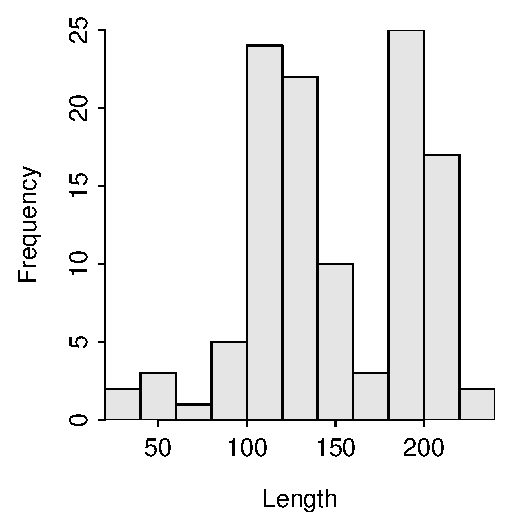
\includegraphics[width=.4\linewidth]{Figs/unnamed-chunk-1-1} 

}



\end{knitrout}
\begin{knitrout}
\definecolor{shadecolor}{rgb}{0.969, 0.969, 0.969}\color{fgcolor}\begin{kframe}
\begin{verbatim}
sex
Female   Male 
  40.4   59.6 
\end{verbatim}
\end{kframe}
\end{knitrout}
\begin{knitrout}
\definecolor{shadecolor}{rgb}{0.969, 0.969, 0.969}\color{fgcolor}\begin{kframe}
\begin{verbatim}
The correlation is 0.772
\end{verbatim}
\end{kframe}

{\centering 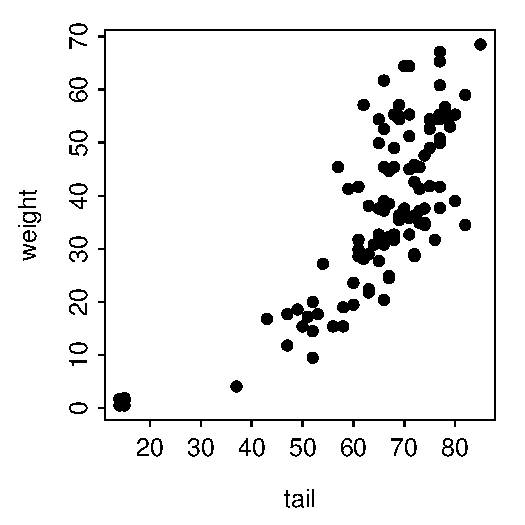
\includegraphics[width=.4\linewidth]{Figs/unnamed-chunk-3-1} 

}



\end{knitrout}
\begin{knitrout}
\definecolor{shadecolor}{rgb}{0.969, 0.969, 0.969}\color{fgcolor}\begin{kframe}
\begin{verbatim}
(Intercept)        tail 
  4.7593879   0.4762164 
The predicted value at a median of 68 is 37.142
The residual is 25 - 28.57 = -3.57
The r-squared value is 0.658
\end{verbatim}
\end{kframe}
\end{knitrout}

\clearpage
\begin{knitrout}
\definecolor{shadecolor}{rgb}{0.969, 0.969, 0.969}\color{fgcolor}\begin{kframe}
\begin{verbatim}
            sex
set          Female Male
  Model          32   47
  Validation     14   21
            sex
set            Female     Male
  Model      31.87719 47.12281
  Validation 14.12281 20.87719
\end{verbatim}
\end{kframe}
\end{knitrout}
\begin{knitrout}
\definecolor{shadecolor}{rgb}{0.969, 0.969, 0.969}\color{fgcolor}\begin{kframe}
\begin{verbatim}
Pearson's Chi-squared test with xtabs(~set + sex, data = df) 
X-squared = 0.0026, df = 1, p-value = 0.9595
\end{verbatim}
\end{kframe}
\end{knitrout}
\begin{knitrout}
\definecolor{shadecolor}{rgb}{0.969, 0.969, 0.969}\color{fgcolor}\begin{kframe}
\begin{verbatim}
Levene's Test for Homogeneity of Variance (center = median)
       Df F value Pr(>F)
group   1  0.4312 0.5127
      112               
\end{verbatim}
\end{kframe}
\end{knitrout}
\begin{knitrout}
\definecolor{shadecolor}{rgb}{0.969, 0.969, 0.969}\color{fgcolor}\begin{kframe}
\begin{verbatim}
 Two Sample t-test with length by sex 
t = -1.87, df = 112, p-value = 0.03205
alternative hypothesis: true difference in means is less than 0 
95 percent confidence interval:
      -Inf -1.834704 
sample estimates:
mean in group Female   mean in group Male 
            139.9783             156.2059 
\end{verbatim}
\end{kframe}
\end{knitrout}

\end{document}
